\documentclass[12pt, 
%twoside
]{article}
\usepackage{braket}
%\usepackage{ctex}%add Chinese supports
\usepackage{upgreek}%add special greek symbols
\usepackage{graphicx}%include figure files
\usepackage{tikz}
\usepackage{wrapfig}
%\usepackage{subfigure}
\usepackage{amsmath}%add special math symbols
\usepackage{amssymb}
\usepackage{bm}%bold math
%\usepackage{xfrac}%add special fraction supports
\usepackage{color}
\usepackage[colorlinks, 
linkcolor=black,
anchorcolor=blue, citecolor=blue, urlcolor=blue]{hyperref}% add hypertext capabilities
\usepackage{geometry}
\geometry{a4paper, centering, scale=0.8}

\usepackage{ntheorem}
\usepackage{fancyhdr}
\pagestyle{fancy}
%\fancyhead[CE]{}
%\fancyhead[CO]{}
%\fancyhead[RO]{\thepage} 
%\fancyhead[LE]{\thepage} 
%\fancyhead[LO]{\leftmark}
%\fancyhead[RE]{\leftmark}

\newtheorem*{thm}{Theorem}
\newtheorem*{proof}{Proof}

\lhead{}
\chead{}
\rhead{\leftmark}
\renewcommand{\headrulewidth}{0.4pt}
\setlength{\headheight}{15pt}

%
%  Created by WW on 06/24/19
%  Copyright © WW. All rights reserved.
%

\begin{document}
	\title{{\bf Introduction to Quantum Mechanics}~\\{\bf\Large ~\\ ---David J. Griffiths}}
	\author{~\\~\\Wei Wang\footnote{Copyright \copyright ~Wei Wang 2019. All rights reserved.}}
	\date{2019-6}
	\maketitle

	\thispagestyle{empty}

	\newpage
	\tableofcontents
	\thispagestyle{empty}% This page is not counted in the page number

	\newpage
	\begin{abstract}
		\addcontentsline{toc}{section}{Abstract}%add Abstract into Contents.
		To review the textbook used in Tongji University --- {\bf\it Introduction to Quantum Mechanics}, written by David J. Griffiths. You can browse through the contents to prepare the final exam of Quantum Mechanics. Also, it will be a good choice for you to prepare the GRE Physics Test...

	\end{abstract}

	{
	\lhead{}
	\chead{}
	\rhead{ABSTRACT}
	}

	\setcounter{page}{1}%start page number counter...

	\newpage

	\lhead{}
	\chead{}
	\rhead{\leftmark}

	\section{Wave Function}
	$\phantom{aaa}$1. General Schr\"odinger equation:
	\begin{equation}\label{eq:1}
		i\hbar \frac{\partial \varPsi}{\partial t}=-\frac{\hbar^2}{2m}\frac{\partial^2\varPsi}{\partial x^2}+V\varPsi
	\end{equation}
	
	p.s., the energy operator is $i\hbar\dfrac{\partial \varPsi}{\partial t}$.
	~\\

	2. Indeterminacy
	~\\

	3. Interpretation:
	Orthodox position = Copenhagen interpretation
	
	Agnostic position
	~\\

	4. \[
		\left\{
		\begin{array}{l}
			{\rm Variance}\\
			{\rm Standard deviation}:~\sigma=\sqrt{<j^2>-<j>^2}\\
		\end{array}
		\right.
		\]
	~\\
		
	5. Normalization
	~\\

	Prove: $\displaystyle\frac{{\rm d}}{{\rm d}t}\int^{\infty}_{-\infty}|\varPsi(x,t)|^2{\rm d}x=0$
	~\\

	Proof:
	$$\frac{{\rm d}}{{\rm d}t}\int_{-\infty}^{\infty}|\varPsi|^2{\rm d}x=\int_{-\infty}^{\infty}\frac{\partial}{\partial t}|\varPsi|^2{\rm d}x$$
	
	and 
	\begin{eqnarray*}
	\frac{\partial}{\partial t}|\varPsi|^2&=&\varPsi^*\frac{\partial \varPsi}{\partial t}+\varPsi\frac{\partial \varPsi^*}{\partial t}~~~~(\rm{Schr\ddot{o}dinger~equation})\\
	&=&\frac{i\hbar}{2m}\left(\varPsi^*\frac{\partial^2\varPsi}{\partial x^2}-\varPsi\frac{\partial^2\varPsi^*}{\partial x^2}\right)\\
	&=&\frac{\partial}{\partial x}\left[\frac{i\hbar}{2m}\left(\varPsi^*\frac{\partial \varPsi}{\partial x}-\varPsi\frac{\partial \varPsi^*}{\partial x}\right)\right]
	\end{eqnarray*}
	
	Q. E. D.
	~\\

	7.\[
		\begin{array}{l}
		<x>=\displaystyle\int\varPsi^*(x)\varPsi{\rm d}x\\
		<p>=\displaystyle\int\varPsi^*\left(\frac{\hbar}{i}\frac{\partial}{\partial x}\right)\varPsi{\rm d}x
		\end{array}
		\]
	~\\

	8. The uncertainty principle:

	\[
		\begin{array}{l}
			p=\dfrac{h}{\lambda}=\hbar k\\
			\sigma_x\sigma_p\geqslant \dfrac{\hbar}{2}
		\end{array}
		\]
	\newpage

	\section{Time-independent Schr\"odinger Equation}
	\subsection{Stationary States}
	Solve Schr\"odinger equation \eqref{eq:1} by the method of separation of variables:
		\[
		\left\{
			\begin{array}{l}
				\displaystyle\frac{{\rm d}\varphi}{{\rm d}t}=-\frac{iE}{\hbar}\varphi\Rightarrow\varphi=\exp(-i\frac{E}{\hbar}t)\\	
				~\\
				\displaystyle-\frac{\hbar^2}{2m}\frac{\partial^2\psi}{\partial x^2}+V\psi=E\psi
			\end{array}
		\right.
		\]	
	and $\displaystyle\hat{H}=\frac{p^2}{2m}+V=-\frac{\hbar^2}{2m}\frac{\partial^2}{\partial x^2}+V~(p\rightarrow\frac{\hbar}{i}\frac{\partial}{\partial x})$, namely:
	\begin{equation}\label{eq:2}
		\hat{H}\varPsi=E\varPsi			
	\end{equation}
	\[
		\varPsi(x,t)=\sum^{\infty}_{n=1}C_n \psi_n(x)e^{-iE_n t/\hbar}
	\]
	\begin{equation}
		\sum_{n=1}^{\infty}\left |C_n\right|^2 =1,
	\end{equation}
	\begin{equation}
		\left<H\right>=\sum_{n=1}^\infty\left|C_n\right|^2E_n.
	\end{equation}
	~\\

	\subsection{Infinite Square Well}
	In a infinite square well:
	\[
		-\frac{\hbar^2}{2m}\frac{\partial^2\psi}{\partial x^2}=E\psi~(0\leqslant x \leqslant a)
	\]
	namely:
	\begin{equation}\label{eq:3}
		\frac{\rm{d^2}\psi}{{\rm d}x^2}=-\frac{2mE}{\hbar}\psi=-k^2\psi 
	\end{equation}
	in which:
	\[
		k=\frac{\sqrt{2mE}}{\hbar}			
	.\]
	We know the solution to equation\eqref{eq:3} is:
	\begin{equation}
		\psi=A\sin kx+B\cos kx.
	\end{equation}
	Boundary conditions:$$\psi(0)=\psi(a)=0,$$we can get $B=0$, and $ka=0,\pm\pi, \pm2\pi...$, namely:
	\[
		k_n=\frac{n\pi}{a},~n=1,2,3...
	\]
	Therefore,$$E_n=\frac{n^2\pi^2\hbar^2}{2ma^2}.$$
	\begin{eqnarray}
		\psi_n(x)&=&\sqrt{\frac{2}{a}}\sin\left (\frac{n\pi}{a}x\right)\\
		\varPsi_n(x,t)&=&\sqrt{\frac{2}{a}}\sin \left (\frac{n\pi}{a}x\right)\exp \left (-i\frac{n^2\pi^2\hbar}{2ma^2}t\right).
	\end{eqnarray}
	~\\

	\subsection{Harmonic Oscillator}
	Hooke's Law:
	\[
		F=-kx=m\frac{{\rm d}^2x}{{\rm d}t^2},
	\]
	namely,
	\[
		\frac{{\rm d}^2 x}{{\rm d}t^2}+\frac{k}{m}x=0,
	\]
	let $\omega=\sqrt{\dfrac{k}{m}}$, so $\displaystyle V(x)=\frac{1}{2}kx^2=\frac{1}{2}m\omega^2x^2$, substituting into eq\eqref{eq:2}, we can get the Schr\"odinger equation of harmonic oscillator:
	\begin{equation}\label{eq:9}
		-\frac{\hbar^2}{2m}\frac{\partial^2}{\partial x^2}\psi+\frac{1}{2}m\omega^2x^2\psi=E\psi.
	\end{equation}
	
	\subsubsection{Ladder Operator}
	1. Hamiltanion: $H=\dfrac{1}{2m}[~p^2+(m\omega x)^2]$, ladder operators: $a_\pm=\dfrac{1}{\sqrt{2\hbar m\omega}}(\mp ip+m\omega x).$
	And we know the commutator of $x$ and $p$ is $[x,p]=i\hbar$, therefore:
	\[
		\left\{
		\begin{array}{l}
			a_{-}a_{+}=\displaystyle \frac{1}{\hbar\omega}H-\frac{i}{2\hbar}[x,p]=\frac{1}{\hbar\omega}H+\frac{1}{2},\\
			~\\
			a_+a_{-}=\displaystyle\frac{1}{\hbar\omega}H-\frac{1}{2}.\\
		\end{array}
		\right.
	\]
	The commutator of $a_{+}$ and $a_{-}$ is: $[a_{-},a_{+}]=a_{-}a_{+}-a_+a_{-}=1$.
	~\\

	\noindent So the Hamiltanion: $$H=\hbar\omega\left (a_\pm a_\mp \pm \frac{1}{2}\right),$$
	and Schr\"odinger equation \eqref{eq:9} become:
	\begin{equation}\label{eq:10}
		\hbar\omega\left (a_\pm a_\mp \pm \frac{1}{2}\right)\psi=E\psi.
	\end{equation}

	\noindent 2. If $H\psi=E\psi$, prove:
	\[
		\left\{
		\begin{array}{l}
			H(a_+\psi)=(E+\hbar\omega)(a_+\psi),\\
			H(a_{-}\psi)=(E-\hbar\omega)(a_{-}\psi).
		\end{array}
		\right.
	\]

\noindent Proof:
\begin{eqnarray*}
	H(a_+\psi)&=&\hbar\omega (a_+a_{-}+\frac{1}{2})(a_+\psi)\\
	&=&\hbar\omega a_+(a_{-}a_++\frac{1}{2})\psi\\
	&=&\hbar\omega a_+(\frac{1}{\hbar\omega}H+1)\psi\\
	&=&a_+(H+\hbar\omega)\psi\\
	&=&a_+(E+\hbar\omega)\psi\\
	&=&(E+\hbar\omega)(a_+\psi)
\end{eqnarray*}

similarly, we can get $$H(a_{-}\psi)=(E-\hbar\omega)(a_{-}\psi).$$

Q. E. D.
~\\

\noindent 3. Ground state $\psi_0$ satisfy: $a_{-}\psi_0=0$, where $a_{-}=\dfrac{1}{\sqrt{2\hbar m\omega}}\left (\hbar\frac{\partial}{\partial x}+m\omega x \right)$, solution:
\[
	\psi_0=\left (\frac{m\omega}{\pi\hbar}\right)^{\frac{1}{4}}e^{-\frac{m\omega}{2\hbar}x^2}.
\]
Substituting $\psi_0$ into Schr\"odinger equation \eqref{eq:10}:
\[
	\hbar\omega(a_+a_{-}+\frac{1}{2})\psi_0=E_0\psi_0 
\]
\[
	\hbar\omega\cdot\frac{1}{2}\psi_0=E_0\psi_0,
\]
Therefore,
\begin{equation}\label{eq:11}
	E_0=\frac{1}{2}\hbar\omega,
\end{equation}
and
\begin{eqnarray*}
	\psi_n&=&A_n(a_+)^n\psi_0=\frac{1}{\sqrt{n!}}(a_+)^n\psi_0~,\\
	E_n&=&(n+\frac{1}{2})\hbar\omega.
\end{eqnarray*}

\noindent 4. Prove $A_n=\dfrac{1}{\sqrt{n!}}.$

\noindent Proof: First, we have to get the Hermitian operator of the raising/lowering ladder operator:
\[
	a_\pm^{\dagger}=a_\mp.
\]

Then, we substitute the $E_n$ back into Schr\"odinger equation \eqref{eq:10}:
\[
	\hbar\omega(a_\pm a_\mp \pm\frac{1}{2})\psi_n=E_n\psi_n=(n+\frac{1}{2})\hbar\omega\psi_n
,\]

namely,
\begin{eqnarray}
	a_+a_{-}\psi_n&=&n\psi_n\\
	a_{-}a_+\psi_n&=&(n+1)\psi_n.
\end{eqnarray}

If $a_+\psi_n=c_n\psi_{n+1}$ and $a_{-}\psi_n=d_n\psi_{n-1}$,
\begin{eqnarray*}
	\int(a_+\psi_n)^*(a_+\psi_n){\rm d}x&=&|c_n|^2\int|\psi_{n+1}|^2{\rm d}x=|c_n|^2\\
	&=&\int(a_{-}a_+\psi_n)^*\psi_n{\rm d}x=(n+1)\int|\psi_n|^2{\rm d}x=n+1	
\end{eqnarray*}

namely: $a_+\psi=\sqrt{n+1}~\psi_{n+1}$, similarly: $a_{-}\psi_n=\sqrt{n}~\psi_{n-1}$. Therefore,
\[
	A_n=\frac{1}{\sqrt{n!}}.
\]

Q. E. D.
~\\

\noindent 5. Prove $\displaystyle\int_{-\infty}^{\infty}\psi_m^*\psi_n=\delta_{mn}$ (Kronecker Delta).

\noindent Proof: 
\begin{eqnarray*}
	\int_{-\infty}^{\infty}\psi_m^*(a_+a_{-})\psi_n{\rm d}x&=&n\int_{-\infty}^{\infty}\psi_m^*\psi_n{\rm d}x\\
	&=&\int_{-\infty}^{\infty}(a_+a_{-}\psi_m)^*\psi_n{\rm d}x=m\int_{-\infty}^{\infty}\psi_m^*\psi_n{\rm d}x.
\end{eqnarray*}

Unless $m\neq n$, $\displaystyle\int_{-\infty}^{\infty}\psi_m^*\psi_n{\rm d}x=0$.

Q. E. D.
~\\

\subsubsection{Analytic Method}
Schr\"odinger equation of harmonic oscillator \eqref{eq:9}:
\[	
	-\frac{\hbar^2}{2m}\frac{\partial^2}{\partial x^2}\psi+\frac{1}{2}m\omega^2x^2\psi=E\psi.
\]
Let $\xi=\sqrt{\dfrac{m\omega}{\hbar}}x$ and $K=\dfrac{2E}{\hbar\omega}$, then:
\[
	\frac{{\rm d}^2\psi}{{\rm d}\xi^2}=(\xi^2-K)\psi.
\]
Solution to this equation:
\[
	\psi_n(x)=\left(\frac{m\omega}{\pi\hbar}\right)^\frac{1}{4}\frac{1}{\sqrt{2^n n!}}H_n(\xi)e^{-\xi^2 /2},
\]
where $H_n(\xi)$ is Hermite polynomials:
\[
	H_0=1,~H_1=2\xi,~H_2=4\xi^2-2.
\]
~\\

\subsection{Free Particle}
Schr\"odinger equation with $V=0$:
\[
	-\frac{\hbar^2}{2m}\frac{\partial^2\psi}{\partial x^2}=E\psi,
\]
then
\[
	\frac{{\rm d}^2\psi}{{\rm d}x^2}=-k^2\psi,~{\rm{where}}~k=\frac{\sqrt{2mE}}{\hbar}.
\]
Solution to this equation:
\[
	\psi(x)=Ae^{ikx}+Be^{-ikx}.
\]
Therefore,
\[
	\varPsi(x,t)=Ae^{ik(x-\frac{\hbar k}{2m}t)},
\]
\[
	k=\pm\frac{\sqrt{2mE}}{\hbar}~\left\{
	\begin{array}{l}
		+:~{\rm right};\\
		-:~{\rm left}.
	\end{array}
	\right.
\]
And $$v_{phase}=v_{quantum}=\frac{\hbar|k|}{2m}=\sqrt{\frac{E}{2m}},$$
$$v_{class}=\frac{2E}{m}=2v_{quantum}.$$
$k$ is continuous spectrum, so
\[
	\varPsi(x,t)=\int_{-\infty}^{\infty}\frac{1}{\sqrt{2\pi}}\phi(k)e^{i(kx-\frac{\hbar k^2}{2m}t)}{{\rm d}}k,
\]
and
\[
	\varPsi(x,0)=\int_{-\infty}^{\infty}\frac{1}{\sqrt{2\pi}}\phi(k)e^{ikx}{\rm d}k,
\]
the coefficient:
\[
	\phi(k)=\int_{-\infty}^{\infty}\frac{1}{\sqrt{2\pi}}\varPsi(x,0)e^{-ikx}{\rm d}x~({\rm Fourier~Transform}),
\]
and
\[
	v_{group}=\frac{{\rm d}\omega}{{\rm d}k}=\frac{\hbar k}{m}=2v_{phase}=v_{class}.
\]

\subsection{Delta-function Potential}
For different $E$:
\[
	\begin{array}{l}
		{\rm boundary~ state:}~E<0;\\
		{\rm scattering~ state:}~E>0.
	\end{array}
\]
For $V(x)=-\alpha \delta(x)$, Schr\"odinger equation:
\[
	-\frac{\hbar^2}{2m}\frac{\partial^2}{\partial x^2}\psi-\alpha\delta(x)\psi=E\psi.
\]

\noindent (1)$~E<0$:

\noindent For $x<0,~V(x)=0$, Schr\"odinger equation:
\[
	\frac{{\rm d}^2 \psi}{{\rm d}x^2}=-\frac{2mE}{\hbar^2}\psi=\kappa^2\psi,~\kappa=\frac{\sqrt{-2mE}}{\hbar}.
\]
Solution to this equation:
\[
	\psi(x)=Ae^{-\kappa x}+Be^{\kappa x}=Be^{\kappa x}~({\rm we~choose} ~A=0,~{\rm for~the~first~term~blows~up~when}~x\rightarrow -\infty),
\]
similarly, $\psi(x)=Fe^{-\kappa x}~(x>0)$.

\noindent The standard boundary conditions for $\psi$:
\[
	\left\{
	\begin{array}{l}
		\psi,~{\rm always~~continuous.}\\
		{\rm d}\psi/{\rm d}x,~{\rm continuous~except~at~point~where~potential~is~infinite.}
	\end{array}
	\right.
\]
Integrating Schr\"odinger equation:
\[
	-\frac{\hbar^2}{2m}\int_{-\varepsilon}^{\varepsilon}\frac{\partial^2\psi}{\partial x^2}{\rm d}x+\int_{-\varepsilon}^{\varepsilon}V(x)\psi{\rm d}x=E\int_{-\varepsilon}^{\varepsilon}\psi{\rm d}x,
\]
when $\varepsilon\rightarrow0$, $\displaystyle\int_{-\varepsilon}^\varepsilon\frac{\partial^2\psi}{\partial x^2}{\rm d}x=\Delta\left(\frac{\partial\psi}{\partial x}\right)$ and $\displaystyle\int_{-\varepsilon}^\varepsilon\psi{\rm d}x=0$,
therefore,
\[
	\Delta\left(\frac{\partial\psi}{\partial x}\right)=\frac{2m}{\hbar^2}\int_{-\varepsilon}^\varepsilon V(x)\psi{\rm d}x=-\frac{2m}{\hbar^2}\int_{-\varepsilon}^\varepsilon\alpha\delta(x)\psi(x){\rm d}x=-\frac{2m\alpha}{\hbar^2}\psi(0).
\]
Now, we know that $B=F$, and $\dfrac{{\rm d}\psi}{{\rm d}x}\Big|_{-}=B\kappa,~\dfrac{{\rm d}\psi}{{\rm d}x}\Big|_+=-B\kappa$, so
\[
	\Delta\left(\frac{{\rm d}\psi}{{\rm d}t}\right)=-2B\kappa=-\frac{2m\alpha}{\hbar^2}B~\Rightarrow~\kappa=\frac{m\alpha}{\hbar^2}.
\]
then,
\[
	E=-\frac{\hbar^2\kappa^2}{2m}=-\frac{m\alpha^2}{2\hbar^2}.
\]
Normalizing $\psi$,
\[
	\int_{-\infty}^\infty|\psi|^2{\rm d}x=2\int_0^\infty|B|^2e^{-2\kappa x}{\rm d}x=\frac{{|B|^2}}{\kappa}=1~\Rightarrow~|B|=\sqrt{\kappa},
\]namely,
\begin{eqnarray*}
	\psi(x)&=&\frac{\sqrt{m\alpha}}{\hbar}e^{-\frac{m\alpha}{\hbar^2}|x|},\\
	E&=&-\frac{m\alpha^2}{2\hbar^2}.
\end{eqnarray*}
~\\

\noindent (2)$~E>0$:

\noindent When $x\neq 0$, Schr\"odinger equation:
\[
	\frac{\partial^2}{\partial x^2}\psi=-k^2\psi, ~k=\frac{\sqrt{2mE}}{\hbar}.
\]
Solution to this equation:
\begin{eqnarray*}
	\psi=Ae^{ikx}+Be^{-ikx},~x<0;\\
	\psi=Fe^{ikx}+Ge^{-ikx},~x>0,
\end{eqnarray*}
using the standard boundary conditions again:
\[
	A+B=F+G,
\]
and
\[
	\frac{{\rm d}\psi}{{\rm d}x}\Big|_{-}=ik(A-B),~\frac{{\rm d}\psi}{{\rm d}x}\Big|_+=ik(F-G),
\]
so
\[
	\Delta\left(\frac{{\rm d}\psi}{{\rm d}x}\right)=ik(F-G-A+B)=-\frac{2m\alpha}{\hbar^2}(A+B).
\]
Consider only the incident wave, namely $G=0$, let $\displaystyle\beta=\frac{m\alpha}{\hbar^2k}$, then
\[
	B=\frac{i\beta}{1-i\beta}A,~F=\frac{1}{1-i\beta}A.
\]
The reflection coefficient $R$ and transmission coefficient $T$:
\[
	R=\frac{|B|^2}{|A|^2},~T=\frac{|F|^2}{|A|^2}.
\]
~\\

\subsection{Finite Square Well}
The potential function of a finite square well is 
\[
	V(x)=\left\{
	\begin{array}{rl}
		-V_0,&~-a\leqslant x\leqslant a\\
		0,&~|x|>a
	\end{array}
	\right.
\]
~\\
\noindent (1)$~E<0$:
~\\\noindent When $x<-a$, Schr\"odinger equation:
\[
	\frac{{\rm d}^2\psi}{{\rm d}x^2}=\kappa^2\psi, ~\kappa=\frac{\sqrt{-2mE}}{\hbar}.
\]
so, $\psi=Be^{\kappa x}$, similarly $\psi=Fe^{-\kappa x}~(x>a)$.

\noindent When $-a<x<a$, Schr\"odinger equation:
\[
	\frac{{\rm d}^2\psi}{{\rm d}x^2}=-l^2\psi, ~l=\frac{\sqrt{2m{E-V_0}}}{\hbar}.
\]
Solution to this equation:
\[
	\psi(x)=C\sin(lx)+D\cos(lx).
\]
We can assume that $\psi(x)$ is an even function, namely:
\[
	\psi(x)=\left\{
	\begin{array}{ll}
		Fe^{-\kappa x}&~,~x>a\\
		D\cos(lx)&~,~0<x<a\\
		\psi(-x)&~,~x<0
	\end{array}
	\right.
\]
Applying the standard boundary conditions:
\[
	Fe^{-\kappa a} = D \cos(la),
\]
\[
	-\kappa F e^{-\kappa a}=-lD\sin(la),
\]
so \[
	\kappa=l\tan(la).
\]
let $z=la$, then
\[
	\tan z=\sqrt{\left(\frac{z_0}{z}\right)^2-1}, ~{\rm where}~z_0=\frac{\sqrt{2mV_0}}{\hbar}a.
\]

\noindent (2)$~E>0$:

\noindent When $x<-a$, Schr\"odinger equation:
\[
	\frac{{\rm d}^2\psi}{{\rm d}x^2}=-k^2\psi, ~k=\frac{\sqrt{2mE}}{\hbar}.
\]
Solution to this equation:
\[
	\psi(x)=Ae^{ikx}+Be^{-ikx},
\]
similarly, $\psi(x)=Fe^{ikx}+Ge^{-ikx}~(x>a)$.
Schr\"odinger equation is the same in the square well, namely
\[
	\psi(x)=C\sin(lx)+D\cos(lx).
\]
Consider only the incident wave, namely $G=0$ ...
\newpage

\section{Formalism}
\subsection{Hilbert Space}
Square-integrable function:
\[
	f(x)~\Rightarrow~\int_a^b|f(x)|^2{\rm d}x<\infty,
\]
all such functions constitutes a vector space {\bf Hilbert Space\footnote{Mathematicians call it $L_2(a,b)$.}}.\\
Inner product of two functions:
\[
	\left<f|g\right>=\int_a^bf(x)^*g(x){\rm d}x,
\]
and
\[
	\left<f|g\right>=\left<g|f\right>^*.
\]
Schwarz inequality:
\begin{equation}\label{eq:14}
	\left|\int_a^bf(x)^*g(x){\rm d}x\right|\leqslant\sqrt{\int_a^b|f(x)|^2{\rm d}x\int_a^b|g(x)|^2{\rm d}x}.
\end{equation}
A set of function is complete is:
\[
	f(x)=\sum_{n=1}^\infty C_nf_n(x),
\]
where $\left<f_m|f_n\right>=\delta_{mn}$ and $C_n=\left<f_n|f\right>$.

\subsection{Observables}
1. Hermitian Operator
\[
	\left<Q\right>=\bra{\psi}\hat{Q}\ket{\psi},
\]
\[
	\left<Q\right>=\left<Q\right>^*,
\]
\[
	\braket{\psi|\hat{Q}\psi}=\braket{\hat{Q}\psi|\psi}.
\]
~\\

\noindent 2. Determined States\\
The value is $q$ when you measure $\hat{Q}$ every time: $\braket{\hat{Q}}=q$, and 
\begin{eqnarray*}
	\sigma^2&=&0\\
	&=&\braket{(\hat{Q}-\braket{Q})^2}\\
	&=&\braket{\psi|(\hat{Q}-\braket{Q})^2\psi}\\
	&=&\braket{(\hat{Q}-q)\psi|(\hat{Q}-q)\psi},
\end{eqnarray*}
therefore: $\hat{Q}\psi=q\psi$.

\subsection{Discrete Spectrum}
1. Prove: Hermitian Operator's eigenvalues are real.\\
Proof: First, we know $\hat{Q}f=qf$, and 
\begin{eqnarray*}
	\braket{f|\hat{Q}f}=\braket{\hat{Q}f|f},
\end{eqnarray*}

and 
\begin{eqnarray*}
	\braket{f|\hat{Q}f}&=&q\braket{f|F},\\
	\braket{\hat{Q}f|f}&=&\braket{qf|f}=\int(qf)^*f{\rm d}x=q^*\int f^*f{\rm d}x=q^*\braket{f|f},
\end{eqnarray*}

therefore: $q=q^*$.

Q. E. D.
~\\

\noindent 2. Eigenfunctions belonging to distinct eigenvalues are orthogonal.~\\

\noindent 3. The eigenfunctions of an observable operator are complete.~\\

\subsection{Continuous Spectrum}
For example, the $\hat{x}$ and $\hat{p}$.\\
1. Dirac orthonormality:
\[
	\braket{f_m|f_n}=\delta(m-n).
\]
\noindent 2. Eigenfunctions are not orthonormal but dirac orthonormal, and not in the Hilbert Space.\\
~\\
\noindent 3. Eigenfunctions of $\hat{x}$ and $\hat{p}$:
\begin{eqnarray*}
	\hat{p}&\rightarrow&f_p=\frac{1}{\sqrt{2\pi\hbar}}e^{ipx/\hbar},~({\rm eigenvalue~is}~p);\\
	\hat{x}&\rightarrow&g_y=\delta(x-y),~({\rm eigenvalue~is}~y).
\end{eqnarray*}
Momentum space wave function:
\begin{eqnarray*}
	\Phi(p,t)&=&\braket{f_p|\Psi(x,t)}\\
	&=&\frac{1}{\sqrt{2\pi\hbar}}\int e^{-ipx/\hbar}\Psi(x,t){\rm d}x.
\end{eqnarray*}
(Position space) wave function:
\begin{eqnarray*}
	\Psi(x,t)&=&\int c(p)f_p{\rm d}p=\frac{1}{\sqrt{2\pi\hbar}}\int e^{ipx/\hbar}\Phi(p,t){\rm d}p.
\end{eqnarray*}

\subsection{The Uncertainty Principle}\label{subsec:3.5}
1. $\sigma_A^2=\braket{(\hat{A}-\braket{A})\psi|(\hat{A}-\braket{A})\Psi}=\braket{f|f}$, similarly $\sigma_B^2=\braket{g|g}$, where $g=\hat{B}-\braket{B}$. For Schwarz inequality:
\[
	\sigma_A^2\sigma_B^2=\braket{f|f}\braket{g|g}\geqslant|\braket{f|g}|^2,
\]
and $|z^2|\geqslant\left|\dfrac{1}{2i}(z-z^*)\right|^2$, so
\[
	\sigma^2_A\sigma^2_B\geqslant(\frac{1}{2i}\left[\braket{f|g}-\braket{g|f}\right])^2=(\frac{1}{2i}\braket{[\hat{A},\hat{B}]})^2.
\]
We know $[x,p]=i\hbar$, so $\sigma_x^2\sigma_p^2\geqslant\left(\dfrac{\hbar}{2}\right)^2$.
~\\

\noindent 2. When $g=cf$ and ${\rm Re}(\braket{f|g})=0$, where $c$ is a constant, the inequality becomes a equality, namely:
\[
	{\rm Re}(c\braket{f|f})=0~\Rightarrow~c=ia 
,\]
so $g=iaf=ia(x-\braket{x})$. For operators $\hat{x}$ and $\hat{p}$, the minimum-uncertainty wave packet is: $$\left(\frac{\hbar}{i}\frac{\partial}{\partial x}-\braket{p}\right)\psi=ia(x-\braket{x})\psi.$$

\noindent 3. The Energy-Time Uncertainty Principle: $\Delta t\Delta E\geqslant \dfrac{\hbar}{2}$.\\
Proof: \[
	\frac{{\rm d}}{{\rm d}t}\braket{Q}=\frac{{\rm d}}{{\rm d}t}\braket{\psi|\hat{Q}\psi}=\braket{\frac{\partial\psi}{\partial t}|\hat{Q\psi}}+\braket{\psi|\frac{\partial\hat{Q}}{\partial t}\psi}+\braket{\psi|\hat{Q}\frac{\partial\psi}{\partial t}}.
\]
And we know the time-dependent Schr\"odinger equation $i\hbar \dfrac{\partial \psi}{\partial t}=\hat{H}\psi$, so:
\[
	\frac{{\rm d}}{{\rm d}t}\braket{Q}=\frac{i}{\hbar}\braket{\hat{H}\psi|\hat{Q}\psi}-\frac{i}{\hbar}\braket{\psi|\hat{Q}\hat{H}\psi}+\braket{\frac{\partial\hat{Q}}{\partial t}}=\frac{i}{\hbar}\braket{[\hat{H},\hat{Q}]}+\braket{\frac{\partial\hat{Q}}{\partial t}}
,\]
if $\hat{Q}$ does not depend explicitly on time, which means $\dfrac{{\partial}\hat{Q}}{\partial t}=0$, we can get:
\begin{equation}\label{eq:15}
	\frac{{\rm d}\braket{Q}}{{\rm d} t}=\frac{i}{\hbar}\braket{[\hat{H},\hat{Q}]}.
\end{equation}
Therefore:
\[
	\sigma_H^2\sigma_Q^2\geqslant(\frac{1}{2i}\braket{[\hat{H},\hat{Q}]})^2=\left(\frac{\hbar}{2}\right)^2\left(\frac{{\rm d}\braket{Q}}{{\rm d} t}\right)^2.
\]
Define
\begin{eqnarray*}
	\Delta E&=&\sigma_H;\\
	\Delta t&=&\frac{\sigma_Q}{|{\rm d}\braket{Q}/{\rm d}t|}, ~{\rm namely:}~\sigma_Q=\left|\frac{{\rm d}\braket{Q}}{{\rm d}t}\right|\Delta t.
\end{eqnarray*}
~\\
\subsection{Dirac Notation}
1. We use a vector in Hilbert Space $\ket{\Im(t)}$ to represent the state of a system (maybe not a function, such as the eigenstates of spin). Then we have $\hat{Q}\ket{f}=f\ket{f}$, so $\ket{\Im(t)}=\displaystyle\int c\ket{f}{\rm d}q$.\\
(1) If $\hat{Q}=\hat{x},$ and $\ket{f}=\ket{x}=g_y$, then
\[
	c=\Psi(x,t)=\braket{x|\Im(t)}.
\]\\
(2) If $\hat{Q}=\hat{p}=\dfrac{\hbar}{i}\dfrac{\partial}{\partial x},$ and $\ket{f}=\ket{p}=f_p$, then
\[
	c=\Phi(p,t)=\braket{p|\Im(t)}.
\]\\
(3) If $\hat{Q}=\hat{H}$, and $\ket{f}=\ket{n}$, then
\[
	c_n=\braket{n|\Im(t)}.
\]

\noindent 2. Operators (represent Observables) are linear transformations:
\[
	\ket{\beta}=\hat{Q}\ket{\alpha},
\]
where $\ket{\alpha}=\sum a_n\ket{e_n}$ and $\ket{\beta}=\sum b_n\ket{e_n}$. And
\[
	\ket{\beta}=\sum b_n\ket{e_n}=\hat{Q}\ket{\alpha}=\sum_n a_n\hat{Q}\ket{e_n},
\]
taking the inner product with $\ket{e_m}$:
\[
	b_m=\sum_n a_n\bra{e_m}\hat{Q}\ket{e_n}=\sum_n Q_{mn} a_n,
\]
namely:
\begin{equation}\label{eq:16}
	Q_{mn}=\bra{e_m}\hat{Q}\ket{e_n}.
\end{equation}
~\\

\noindent 3. Projection Operator: $\hat{P}=\ket{\alpha}\bra{\alpha}$, where $\ket{\alpha}$ is a normalized vector.
\[
	{\rm e.~g.~}~\hat{P}\ket{\beta}=\ket{\alpha}\braket{\alpha|\beta}=\braket{\alpha|\beta}\ket{\alpha},
\]
where $\braket{\alpha|\beta}$ is the projection of $\ket{\beta}$ in the direction of $\ket{\alpha}$. Therefore, we know:
\[
	\sum_n \ket{e_n}\bra{e_n}=1,
\]
for $\sum_n \ket{e_n}\braket{e_n|\beta}=\ket{\beta}$.
~\\

\noindent 4. Commutator's property: 
\begin{equation}\label{eq:17}
	[AB,C]=A[B,C]+[A,C]B.
\end{equation}

\newpage

\subsection{Physical Significance of Commutators}

\begin{thm}
	If operator $\hat{H}$ and $\hat{Q}$ share a complete set of eigenfunctions, then these two operators commute with each other.
\end{thm}
\begin{proof}
	If the two operators share a complete set of eigenfunctions $\{\phi_n\}$,
	$$\hat{H}\phi_n=E_n\phi_n,~\textit{and}~\hat{Q}\phi_n=q_n\phi_n,$$
we can get 
	$$[\hat{H},\hat{Q}]\phi_n=\hat{H}\hat{Q}\phi_n-\hat{Q}\hat{H}\phi_n=E_nq_n\phi_n-q_nE_n\phi_n=0.$$
As $\{\phi_n\}$ are complete, i.e., $\forall\varPhi\in$ Hilbert Space $L_2(a,b)$, $\exists c_n$ satisfy $\varPhi=\sum c_n\phi_n$, we can get
	$$[\hat{H},\hat{Q}]\varPhi_n=\sum c_n[\hat{H},\hat{Q}]\phi_n=0.$$
	So the two operators commute with each other.\hfill$\square$

\end{proof}

\begin{thm}[converse]
	If two operators commute with each other, i.e, $[\hat{H}, \hat{Q}]=0$, operator $\hat{H}$ and $\hat{Q}$ share a complete set of eigenfunctions.
\end{thm}
\begin{proof}
	If ${\phi_n}$ is a complete set of eigenfunctions of operator $\hat{H}$ (nondegenerate), namely,
	$$\hat{H}\phi_n=E_n\phi_n,$$
	and if $[\hat{H},\hat{Q}]=0$, we can get
	$$\hat{H}\hat{Q}\phi_n-\hat{Q}\hat{H}\phi_n=0\Rightarrow\hat{H}\hat{Q}\phi_n=E_n\hat{Q}\phi_n.$$
	So $\hat{Q}\phi_n$ is also an eigenfunction of operator $\hat{H}$ corresponding to the same eigenvalue $E_n$, which means $\hat{Q}\phi_n$ and $\phi_n$ differ only by a constant, i.e.,
	$$\hat{Q}\phi_n=c_n\phi_n.$$
	So $\{\phi_n\}$ are also the eigenfunctions of operator $\hat{Q}$. And we can get the similar results for degenerate cases.\hfill$\square$
\end{proof}

\noindent{\bf Conclusion}:
~\\

$[\hat{H},\hat{Q}]=0$ is the {\bf Necessary and Sufficient Condition} of that operator $\hat{H}$ and $\hat{Q}$ share a complete set of eigenfunctions.
~\\

$[\hat{H},\hat{Q}]=0$ means these two observables can {\bf be measured simultaneously}, or in another word, these two observables can {\bf have determinate values at the same time}. (cf. section \ref{subsec:3.5} The Uncertainty Principle).

\newpage

\section{Quantum Mechanics in Three Dimensions}
\subsection{Spherical Coordinates}
Schr\"odinger equation $i\hbar\dfrac{\partial \varPsi}{\partial t}=\hat{H}\varPsi$, and $\hat{p}=\dfrac{\hbar}{i}\nabla$, namely:
\begin{equation}\label{eq:18}
	i\hbar\frac{\partial\varPsi}{\partial t}=-\frac{\hbar^2}{2m}\nabla^2\varPsi+V\varPsi.
\end{equation}
The time-independent schr\"odinger equation:
\begin{equation}\label{eq:19}
	-\frac{\hbar^2}{2m}\nabla^2\psi+V\psi=E\psi.
\end{equation}
In spherical coordinates:
\[
	\nabla^2=\frac{1}{r^2}\frac{\partial}{\partial t}\left(r^2\frac{\partial}{\partial r}\right)+\frac{1}{r^2}\frac{1}{\sin\theta}\frac{\partial}{\partial\theta}\left(\sin\theta\frac{\partial}{\partial\theta}\right)+\frac{1}{r^2}\frac{1}{\sin^2\theta}\frac{\partial^2}{\partial \phi^2},
\]
where $\theta$ is the polar angle and $\phi$ is the azimuthal angle. Solve Schrödinger equation\eqref{eq:19} by the method of separation of variables:
\[
	\psi(x,\theta,\psi)=R(r)Y(\theta,\psi),~{\rm and~}Y(\theta,\psi)=\varTheta(\theta)\Phi(\phi),
\]
and the separation constant is $l(l+1)$ and $m^2$ respectively. Therefore:
\[
	\Phi(\psi)=e^{im\phi},
\]
and we know $\Phi(\phi+2\pi)=\Phi(\phi)$, so $m=0,\pm1,\pm2...$
And \[
	\varTheta(\theta)=AP_l^m(\cos\theta),
\]
so $l>0$, and $l\geqslant|m|$. For $\forall l=0,1,2...$, $m=\underbrace{-l,-l+1,\cdots-1,0,1,\cdots l-1,l}_{2l+1~{\rm terms}}$.\\
The normalization condition of angular equation is:
\[
	\int_0^{2\pi}\int_0^{\pi}|Y|^2\sin\theta{\rm d}\theta{\rm d}\phi=1,
\]
and the normalized angular wave function are called {\bf Spherical Harmonics}:
\[
	Y_l^m(\theta,\phi)=\varepsilon\sqrt{\frac{(2l-a)}{4\pi}\frac{(l-|m|)!}{(l+|m|)!}}e^{im\phi}P_l^m(\cos\theta),
\]
where $\varepsilon=(-1)^m$ when $m\geqslant0$, and $\varepsilon=1$ when $m\leqslant0$. And
\[
	\int_0^{2\pi}\int_0^{2\pi}Y_l^mY_{l'}^{m'}\sin\theta{\rm d}\theta{\rm d}\phi=\delta_{ll'}\delta_{mm'},
\]
where $l$ is called azimuthal quantum number and $m$ is called magnetic quantum number.
\\

\noindent To solve the radial equation, let $u(r)=rR(r)$, so that the normalization condition becomes:
\[
	\int_0^\infty|R(r)|^2 r^2{\rm d}r=1~\Rightarrow~\int_0^\infty|u|^2{\rm d}r=1
,\]
and the radial function becomes:
\begin{equation}\label{eq:20}
	-\frac{\hbar^2}{2m}\frac{{\rm d}^2u}{{\rm d}r^2}+\left[V+\frac{\hbar^2}{2m}\frac{l(l+1)}{r^2}\right]u=Eu,
\end{equation}
we can see that there exists an effective potential:
\[
	V_{\rm eff}=\frac{\hbar^2}{2m}\frac{l(l+1)}{r^2}.
\]
Then We can get the solution to the radial equation:
\[
	R(r)=Aj_l(kr),~k=\frac{\sqrt{2mE}}{\hbar},
\]
where $j_l(x)$ is the spherical Bessel function of order $l$. And the boundary conditions:
\begin{eqnarray*}
	R(a)&=&0;\\
	ka&=&\beta_{nl},
\end{eqnarray*}
in which $\beta_{nl}$ is the $n$th zero of the $l$th spherical Bessel function.

\subsection{Hydrogen Atom}
1. For hydrogen atom, potential energy:
\[
	V(r)=-\frac{e^2}{4\pi\varepsilon_0}\frac{1}{r},
\]
and the radial equation\eqref{eq:20} says:
\[
	-\frac{\hbar^2}{2m}\frac{{\rm d}^2 u}{{\rm d}r^2}+\left[-\frac{e^2}{4\pi\varepsilon_0}\frac{1}{r}+\frac{\hbar^2}{2m}\frac{l(l+1)}{r^2}\right]u=Eu.
\]
Let $\kappa=\dfrac{\sqrt{-2mE}}{\hbar}$, and $\rho=\kappa r$, $\rho_0=\dfrac{me^2}{2\pi\varepsilon_0\hbar^2\kappa}$, we can get the famous {\bf Bohr Formula}:
\begin{equation}
	E_n=-\left[\frac{m}{2\hbar^2}\left(\frac{e^2}{4\pi\varepsilon_0}\right)^2\right]\frac{1}{n^2}=\frac{E_1}{n^2},~n=1,2,3,\dots
\end{equation}
and from $\rho_0=2n$ and $n\equiv j_{max}+l+1$, we can derive that
\[
	\kappa=\left(\frac{me^2}{4\pi\varepsilon_0\hbar^2}\right)\frac{1}{n}=\frac{1}{an}, ~{\rm and}~\rho=\frac{r}{an},
\]
and the so-called {\bf Bohr Radius}:
\[
	a=\frac{4\pi\varepsilon_0\hbar^2}{me^2}\approx 0.529\times10^{-10}m.
\]
Also $l=0,1,\cdots n-1$, the total degeneracy of energy level $E_n$ is $\displaystyle d(n)=\sum_{l=0}^{n-1}(2l+1)=n^2$. Therefore, the normalized hydrogen wave function is (associated Laguerre polynomial) ...
~\\

\noindent 2. The spectrum of hydrogen:
\[
	E_\gamma=E_i-E_f=E_1\left(\frac{1}{n_i^2}-\frac{1}{n_f^2}\right),
\]
namely,
\[
	h\nu=E_1\left(\frac{1}{n_i^2}-\frac{1}{n_f^2}\right), ~{\rm where}~\hbar=\frac{h}{2\pi},
\]
i.e.,
\[
	\frac{1}{\lambda}=R\left(\frac{1}{n_f^2}-\frac{1}{n_i^2}\right),~{\rm where~the~{\bf Rydberg~Constant}~is}~R=\frac{m}{4\pi c\hbar^3}\left(\frac{e^2}{4\pi\varepsilon_0}\right)^2.
\]
And 
\begin{table}[h]
	\centering
	\begin{tabular}{ccc}
	\hline\hline
		$n_f$&&Spectrum series\\
	\hline
		1&&Lyman\\
		2&&Balmer\\
		3&&Paschen\\
	\hline\hline
	\end{tabular}
\end{table}
~\\

\subsection{Angular Momentum}
Angular momentum: $\vec{L}=\vec{r}\times\vec{p}$, and 
\[
	L_x=yp_z-zp_y,~L_y=zp_x-xp_z,~L_z=xp_y-yp_x.
\]
We can derive that
\[
	[r_i,r_j]=[p_i,p_j]=0,
\]
and \[
	[r_i, p_j]=i\hbar\delta_{ij}=-[p_i,r_j].	
\]
Therefore, $[L_x, L_y]=i\hbar L_z$ ...
And
\[
	\sigma_{L_x}^2\sigma_{L_y}^2\geqslant\left(\frac{1}{2i}\braket{i\hbar L_z}\right)^2=\frac{\hbar^2}{4}\braket{L_z}^2,
\]
namely, $\sigma_{L_x}\sigma_{L_y}\geqslant\dfrac{\hbar}{2}|\braket{L_z}|$ ...
And \[
	[L^2,L_x]=[L^2,L_y]=[L^2,L_z]=0,
\]
namely, $[L^2,\vec{L}]=0$.\\
If 
\begin{eqnarray*}
	L^2f=\lambda f;\\
	L_zf=\mu f,
\end{eqnarray*}
let $L_\pm=L_x\pm iL_y$, we know $[L_z,L_\pm]=\pm\hbar L_\pm$ and $[L^2, L_\pm]=0$, then
\begin{eqnarray*}
	L^2(L_\pm f)&=&\lambda(L_\pm f);\\
	L_z(L_\pm f)&=&(\mu+\hbar)(L_\pm f).
\end{eqnarray*}
Then $L^2=L_\pm L_\mp +L_z^2\mp\hbar L_Z$, we can derive that:
\begin{eqnarray*}
	L^2f_l^m&=&\hbar^2l(l+1)f_l^m;\\
	L_zf_l^m&=&\hbar mf_l^m,
\end{eqnarray*}
where $m=-l, -l+1,\cdots l-1,l$ and $l=0,1/2,1,3/2\dots$, also
\begin{equation}\label{eq:22}
	L_\pm f_l^m=\hbar\sqrt{l(l+1)-m(m\pm1)}f_l^{m\pm 1}.
\end{equation}~\\

\subsection{Spin}
Similarly, \[
	[S_x,S_y]=i\hbar S_z,~[S_y,S_z]=i\hbar S_x,~[S_z,S_x]=i\hbar S_y.
\]
Also
\begin{eqnarray*}
	S^2\ket{sm}&=&\hbar^2s(s+1)\ket{sm};\\
	S_z\ket{sm}&=&\hbar m\ket{sm},
\end{eqnarray*}
where $\ket{sm}$ is the eigenstate of spin, and it is not a function, so we use a vector to represent it.
Let $S_\pm=S_x\pm iS_y$, then
\begin{equation}
	S_\pm\ket{sm}=\hbar\sqrt{s(s+1)-m(m\pm1)}\ket{s(m\pm1)},
\end{equation}
where $s=0,1/2,1,3/2\dots$ and $m=-s, -s+1,\cdots s-1,s$.\\
For $s=1/2$, there are just two eigenstate $\displaystyle\ket{\frac{1}{2}~\frac{1}{2}}$ and $\displaystyle\ket{\frac{1}{2}~(-\frac{1}{2})}$, which we call spin up ($\uparrow$) and spin down ($\downarrow$). Then we can use spinor to represent the general state:
\[
	\chi= \begin{pmatrix}
		a\\b
	\end{pmatrix}=a\chi_++b\chi_{-}
,\]
in which $\chi_+= \begin{pmatrix}
	1\\0
\end{pmatrix}~(\uparrow)$ and $\chi_{-}= \begin{pmatrix}
	0\\1
\end{pmatrix}~(\downarrow)$. Therefore:
\[
	S^2\chi_+=S^2\ket{\frac{1}{2}~\frac{1}{2}}=\hbar^2\frac{1}{2}\times\frac{3}{2}\ket{\frac{1}{2}~\frac{1}{2}}=\frac{3}{4}\hbar^2\chi_+
,\]
similarly, $S^2\chi_{-}=\frac{3}{4}\hbar^2\chi_{-}$, so
\[
	S^2=\frac{3}{4}\hbar^2 \begin{pmatrix}
		1&0\\0&1
	\end{pmatrix}.
\]
And $S_z\chi_+=\frac{1}{2}\hbar\chi_+$, $S_z\chi_{-}=-\frac{1}{2}\hbar\chi_{-}$, so
\[
	S_z=\frac{\hbar}{2} \begin{pmatrix}
		1&0\\0&-1
	\end{pmatrix}.
\]
Also $S_+\chi_+=S_{-}\chi_{-}=0$, $S_+\chi_{-}=\hbar\chi_+$, $S_{-}\chi_+=\hbar\chi_{-}$, so
\[
	S_+=\hbar \begin{pmatrix}
		 0&1\\0&0
	\end{pmatrix},~S_{-}=\hbar \begin{pmatrix}
		0&0\\1&0
	\end{pmatrix},
\]
then, we can use $S_\pm=S_x\pm iS_y$ to get $S_x$ and $S_y$.\\
Therefore, $$\vec{S}=\frac{\hbar}{2}\sigma,$$where $\sigma$ is called {\bf Pauli Spin Matrix}:
\[
	\sigma_x= \begin{pmatrix}
		0&1\\1&0
	\end{pmatrix},~\sigma_y= \begin{pmatrix}
		0&-i\\i&0
	\end{pmatrix},~\sigma_z= \begin{pmatrix}
		1&0\\0&-1
	\end{pmatrix}.
\]
~\\
Magnetic dipole momentum 
\[
	\vec{\mu}=\gamma\vec{S},
\]
and Hamiltanion 
\[
	H=-\vec{\mu}\cdot\vec{B}=-\gamma\vec{B}\cdot\vec{S}.
\]
...\\

\noindent Two spin-1/2 particle:
\[
	s=1~({\rm triplet})~\left\{
	\begin{array}{l}
		\ket{11}=\uparrow\uparrow ,\\
		\ket{10}=\dfrac{1}{\sqrt{2}}(\uparrow\downarrow+\downarrow\uparrow) ,\\
		\ket{1-1}=\downarrow\downarrow,
	\end{array}\right.
\]
and
\[
	s=0~(\rm singlet):~\ket{00}=\frac{1}{\sqrt{2}}(\uparrow\downarrow-\downarrow\uparrow).
\]
\newpage
\section{Identical Particles}
\subsection{Two-Particle System}
Wave function $\varPsi(\vec{r}_1,\vec{r}_2,t)$ satisfy Schr\"odinger equation:
\[
	i\hbar\frac{\partial\varPsi}{\partial t}=H\varPsi,
\]
in which $\displaystyle H=-\frac{\hbar^2}{2m}\nabla^2_1-\frac{\hbar^2}{2m}\nabla_2^2+V(\vec{r}_1,\vec{r}_2,t).$\\~

\noindent1. Distinguishable particles:
\[
	\varPsi(\vec{r}_1,\vec{r}_2)=\varPsi_a(\vec{r}_1)\varPsi_b(\vec{r}_2).
\]\\
2. Indistinguishable particles:
\[
	\varPsi_\pm(\vec{r}_1,\vec{r}_2)=A[\varPsi_a(\vec{r}_1)\varPsi_b()\vec{r}_2)\pm\varPsi_a(\vec{r}_2)\varPsi_b(\vec{r}_1)],
\]
where "$+$" represents {\bf Bosons} (integer spin), and "$-$" represents {\bf Fermions} (half integer spin).\\

\noindent 3. Pauli Exlusion Principle: if $\varPsi_a=\varPsi_b$, then $\varPsi_{-}(\vec{r}_1,\vec{r}_2)=0$.\\

\noindent 4. Exchange symmetric/antisymmetric: $\varPsi(\vec{r}_1,\vec{r}_2)=\pm\varPsi(\vec{r}_2,\vec{r}_1)$.\\

\noindent 5. Exchange force:
\[
	\braket{(x_1-x_2)^2}_\pm=\braket{(x_1-x_2)^2}_d\mp 2\left|\braket{x}_{ab}\right|^2,
\]
where $\braket{(x_1-x_2)^2}_d=\braket{x^2}_a+\braket{x^2}_b-2\braket{x}_a\braket{x}_b$, and $\displaystyle\braket{x}_{ab}=\int x\varPsi_a^*\varPsi_b{\rm d}x.$ Therefore, 
\begin{eqnarray*}
	 &\rm the~upper~sign&\rm :~bosons~\Rightarrow~bonding,\\
	 &\rm the~lower~sign&\rm :~fermion~\Rightarrow~antibonding.
\end{eqnarray*}
For electrons: the complete state is
\[
	\varPsi(\vec{r})\chi(\vec{s}),
\]
where $\varPsi(\vec{r})$ is antisymmetric with respect to exchange. So if $\chi(\vec{s})$ is singlet (antisymmetric), the complete state is symmetric which should lead to {\it bonding} ({\bf Covalent Bond}). And if $\chi(\vec{s})$ is triplet (symmetric), it should lead to {\it antibonding}.
\newpage

\section{Time-Independent Perturbation Theory}
\subsection{Nondegenerate Perturbation}
1. First-Order Theory:
\begin{equation}\label{eq:24}
	E^1_n=\bra{\psi_n^0}H'\ket{\psi_n^0},
\end{equation}
and $\psi^1_n=\sum_{m\neq n}C_m^{(n)}\psi_m^0$, then
\[
	\psi^1_n=\sum_{m\neq n}\frac{\bra{\psi_m^0}H'\ket{\psi_n^0}}{(E_n^0-E_m^0)}\psi_m^0.
\]
2. Second-Order Energies:
\begin{eqnarray*}
	E_n^2&=&\bra{\psi_m^0}H'\ket{\psi_n^1}\\
	&=&\sum_{m\neq n}\frac{\bra{\psi_m^0}H'\ket{\psi_n^0}\bra{\psi_n^0}H'\ket{\psi_m^0}}{(E_n^0-E_m^0)}\\
	&=&\sum_{m\neq n}\frac{\left|\bra{\psi_m^0}H'\ket{\psi_n^0}\right|^2}{(E_n^0-E_m^0)}.
\end{eqnarray*}

\subsection{Degenerate Perturbation}
The matrix elements of $H'$: $W_{ij}=\bra{\psi_i^0}H'\ket{\psi_j^0}$. And $W_{ab}=W_{ba}^*=\bra{\psi^0_a}H'\ket{\psi_b^0}$, then
\[
	E^1_\pm=\frac{1}{2}\left[W_{aa}+W_{bb}\pm\sqrt{(W_{aa}-W_{bb})^2+4|W_{ab}|^2}\right].
\]
Matrix form:
\[
	\begin{pmatrix}
		W_{aa}&W_{ab}\\W_{ba}&W_{bb}
	\end{pmatrix} \begin{pmatrix}
		\alpha\\\beta
	\end{pmatrix}=E^1 \begin{pmatrix}
		\alpha\\\beta
	\end{pmatrix}.
\]
If $[A,H']=0$, $Af=\mu f$, and we use $f$ as $\psi_n^0$, the $W$ matrix will automatically be diagonal.
~\\

\subsection{Fine Structure of Hydrogen}
Two distinct mechanisms: {\bf Relativistic Correction} and {\bf Spin-Orbit Coupling}. And the famous $Fine Structure Constant$:
\[
	\alpha=\frac{e^2}{4\pi\varepsilon_0\hbar c}\approx\frac{1}{137}.
\]
\subsubsection{Relativistic Correction}
The relativistic kinetic energy:
\begin{eqnarray*}
	T&=&\sqrt{p^2 c^2+m^2c^4}-mc^2\\
	&=&mc^2(\sqrt{1+\left(\frac{p}{mc}\right)^2}-1)\\
	&=&mc^2(\frac{1}{2}\left(\frac{p}{mc}\right)^2-\frac{1}{8}\left(\frac{p}{mc}\right)^4+\dots)\\
	&=&\frac{p^2}{2m}-\frac{p^4}{8m^3c^2}+\dots
\end{eqnarray*}
so $H^1_r=-\dfrac{p^4}{9m^3c^2}$. With equation \eqref{eq:24},
\[
	E_n^1=\braket{H_r^1}=-\frac{1}{8m^3c^2}\bra{\psi}p^4\ket{\psi}=-\frac{1}{8mc^3c^2}\braket{p^2\psi|p^2\psi},
\]
and $p^2\psi=2m(E-V)\psi$ (Schr\"odinger equation), then
\[
	E^1_n=-\frac{1}{2mc^2}\braket{(E-B)^2}=-\frac{1}{2mc^2}(E^2-2E\braket{V}+\braket{V^2}).
\]
For hydrogen atom:
\[
	\left<\frac{1}{r}\right>=\frac{1}{n^2a},
\]
where $a$ is Bohr radius.
~\\

\subsubsection{Spin-Orbit Coupling}
From electron's point of view:
\[
	\begin{array}{l}
		(1)~{\rm proton~circling~around~electron}~\Rightarrow~\vec{B}~\Rightarrow~{\rm orbit},\\
		(2)~{\rm electron~spin}~\Rightarrow~\vec{\mu}~\Rightarrow~{\rm spin},
	\end{array}
\]
(1) The magnetic field:
\[
	\vec{B}=\frac{\mu_0}{4\pi}\int\frac{I}{r^2}{\rm d}\vec{l}=\frac{\mu_0I}{2r},
\]
where $I=\dfrac{e}{T}$, $L=rp=rm\dfrac{2\pi r}{T}=\dfrac{2\pi m r^2}{T}$. Therefore:
\[
	\vec{B}=\frac{1}{4\pi\varepsilon_0}\cdot\frac{e}{mc^2r^3}\vec{L}.
\]
(2) The magnetic dipole moment:
\[
	\mu=I\cdot\pi r^2, ~I=\frac{q}{T},~S=\frac{2\pi m r^2}{T},
\]
where $S$ is the spin angular momentum. Therefore the {\bf Gyromagnetic Ratio}:
\[
	\gamma=\frac{\mu}{S}=\frac{q}{2m},
\]
namely $\vec{\mu}=\left(\dfrac{q}{2m}\right)\vec{S}$. For electrons, it actually is $\vec{\mu}=-\dfrac{e}{m}\vec{S}$.\\
Therefore,
\begin{eqnarray*}
	H'_{\rm so}=-\vec{\mu}\cdot\vec{B}=\left(\frac{e^2}{4\pi\varepsilon_0}\right)\frac{1}{m^2c^2r^3}\vec{S}\cdot\vec{L},
\end{eqnarray*}
after making a appropriate correction, it becomes:
\[
	H'_{\rm so}=\left(\frac{e^2}{8\pi\varepsilon_0}\right)\frac{1}{m^2c^2r^3}\vec{S}\cdot\vec{L}.
\]
The total angular momentum $\vec{J}=\vec{L}+\vec{S}$. The Hamiltanion no longer commutes with $\vec{L}$ and $\vec{S}$, $H'_{\rm so}$ does commutes with $L^2$, $S^2$ and $\vec{J}$, and 
\[
	\vec{L}\cdot\vec{S}=\frac{1}{2}(J^2-L^2-S^2)=\frac{\hbar^2}{2}[j(j+1)-l(l+1)-s(s+1)].
\]

\subsubsection{Zeeman Effect}
For a single electron, the perturbation is \[
	H'_Z=-(\vec{\mu}_l+\vec{\mu}_s)\cdot\vec{B}_{\rm ext},
\]
where $\vec{\mu}_l=-\dfrac{e}{2m}\vec{L}$ is the dipole momentum associated with orbital motion, and $\vec{\mu}_s=-\dfrac{e}{m}\vec{S}$ is the magnetic dipole momentum associated with electron spin. Then
\[	
	H'_Z=\frac{e}{2m}(\vec{L}+2\vec{S})\cdot\vec{B}_{\rm ext}.
\]
(1) When $B_{\rm ext}\ll B_{\rm int}$, the fine structure dominates, $H'_z$ is perturbation. Then
\[
	E_Z^1=\frac{e}{2m}\vec{B}_{\rm ext}\cdot\braket{\vec{L}+2\vec{S}}.
\]

\begin{wrapfigure}{r}{.4\textwidth}
\hspace{0.8cm}
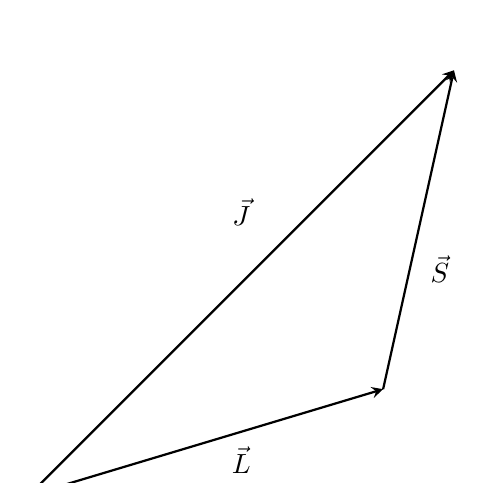
\begin{tikzpicture}[scale=0.9]
	\coordinate (A) at (-6,-4);
	\coordinate (B) at (0,2);
	\coordinate (C) at (-1,-2.5);
	\draw[thick, -stealth] (A)--(B);
	\draw[thick, -stealth] (A)--(C);
	\draw[thick, -stealth] (C)--(B);
	\node at (-3,0) {$\vec{J}$};
	\node at (-3,-3.5) {$\vec{L}$};
	\node at (-0.2,-0.8) {$\vec{S}$};
\end{tikzpicture}
\caption{$\vec{J}=\vec{L}+\vec{S}$ is a constant.}
\label{fg:1}
\end{wrapfigure}

\noindent We know that $\vec{L}+2\vec{S}=\vec{J}+\vec{S}$, and the total angular momentum $\vec{J}$ is a constant (see Figure \ref{fg:1}), so the average value of $\vec{S}$:
\[
	\vec{S}_{\rm ave}=\frac{(\vec{S}\cdot\vec{J})}{J^2}\vec{J}.
\]
Therefore,
\begin{eqnarray*}
	\braket{\vec{L}+2\vec{S}}&=&\braket{(1+\frac{\vec{S}\cdot\vec{J}}{J^2})\vec{J}}\\
	&=&\left[1+\frac{j(j+1)+s(s+1)-l(l+1)}{2j(j+1)}\right]\braket{\vec{J}}\\
	&=&g_J\braket{\vec{J}},
\end{eqnarray*}
where $g_J$ is known as {\bf Land\'{e} g-factor}.
Then
\[
	E^1_Z=\frac{e}{2m}g_J\vec{B}_{\rm ext}\cdot\braket{\vec{J}},
\]
if we choose $\vec{B}_{\rm ext}$ along $z$-axis, then
\[
	E_Z^1=\frac{e}{2m}g_JB_{\rm ext}\hbar m_j=\mu_B g_JB_{\rm ext}m_j,
\]
where $\mu_B=\dfrac{e\hbar}{2m}$ is the so-called {\bf Bohr Magneton}.\\

\noindent (2) When $B_{\rm ext}\gg B_{\rm int}$ ...\\

\noindent (3) Neither $H'_Z$ or $H'_{\rm fs}$ dominates, then $H'=H'_Z+H'_{\rm fs}$ ...
\newpage

\section{Variational Principle}
Prove:
\[	
	E_{\rm gs}\leqslant\bra{\psi}H\ket{\psi}\equiv\braket{H}.
\]
Poof: we can express $\psi$ as $\psi=\sum C_n\psi_n$, then
\[
	1=\braket{\psi|\psi}=\left<\sum C_m\psi_m|\sum C_n\psi_n\right>=\sum_m\sum_n C_m^*C_n=\sum_n\left|C_n\right|^2,
\]

therefore
\[
	\braket{H}=\sum_nE_n\left|C_n\right|^2\geqslant\sum_nE_{\rm gs}\left|C_n\right|^2=E_{\rm gs}.
\]

The most common "trial" wave function is
\[
	\psi(x)=Ae^{-bx^2},
\]

and the ground state hydrogen atom wave function
\[
	\psi_{100}=\frac{1}{\sqrt{\pi a^3}}e^{-r/a}.
\]

\section{WKB Approximation}
The classic momentum of a particle is $p(x)\equiv\sqrt{2m[E-V(x)]}$, then
\[
	\psi(x)\approx\frac{C}{\sqrt{p(x)}}e^{\pm\frac{i}{\hbar}\int p(x){\rm d}x}.
\]

\end{document}


